\chapter{Análise Teórica}
\label{ch:anal_teo} % This how you label a chapter and the key (e.g., ch:into) will be used to refer this chapter ``Introduction'' later in the report. 
% the key ``ch:into'' can be used with command \ref{ch:intor} to refere this Chapter.

\section{Bubble Sort}
\label{sec:bubble_sort_teo}

O Bubble Sort, também conhecido como "Ordenação por bolha" ou "Ordenação por flutuação", é um dos algoritmos de ordenação mais simples.

Neste algoritmo, são realizadas comparações entre os dados armazenados em um vetor de tamanho \( n \). Cada elemento na posição \( i \) é comparado com o elemento na posição \( i+1 \). Quando a ordenação procurada — seja ela crescente ou decrescente — é encontrada, ocorre uma troca de posições entre os elementos.

O algoritmo executa dois laços principais:

\begin{enumerate}
	\item[\textbf{1.}] O primeiro laço percorre a quantidade de elementos do vetor:
	      \begin{verbatim}
    for (j = 1; j <= n; j++)
    \end{verbatim}

	\item[\textbf{2.}] O segundo laço, que está dentro do primeiro, percorre da primeira à penúltima posição do vetor:
	      \begin{verbatim}
    for (i = 0; i < n - 1; i++)
    \end{verbatim}
\end{enumerate}


\begin{figure}[!ht]
	\centering
	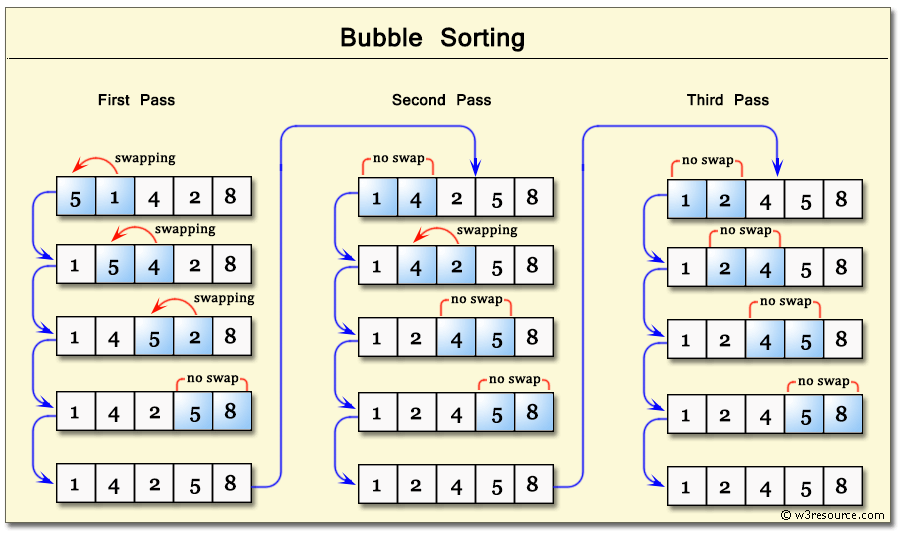
\includegraphics[scale=0.3]{figures/bubble/bubbleDiagram.png}
	\caption{Diagrama exemplo de um Bubble Sort}
	\label{fig:bubble_sort_example}
\end{figure}
\FloatBarrier

\subsection{Bubble Sort Iterativo}

Dessa forma, estabelecemos o pseudocódigo de sua versão iterativa como:

\begin{algorithm}
	\caption{Bubble Sort}
	\label{algo:bubble_sort_it}
	\begin{algorithmic}[1]
		\Require{Lista $A = A_1, A_2, \ldots, A_n$}
		\Ensure{Lista $A$ ordenada}
		\Statex
		\Function{BubbleSort}{$A$}
		\For{$j \gets 1$ to $n - 1$}
		\For{$i \gets 0$ to $n - 2$}
		\If {$A[i] > A[j + 1]$}
		\State \textbf{troque} $i$ por $j$ em $A$
		\EndIf
		\EndFor
		\EndFor
		\EndFunction
	\end{algorithmic}
\end{algorithm}
\FloatBarrier

\subsection{Bubble Sort Recursivo}

Para sua versão recursiva, vamos analisar o algoritmo em dois casos. Quando uma lista tem no máximo $1$ elemento, ela está ordenada, então esse será o caso base. Para o caso recursivo, pelo teorema da recursão podemos assumir que a função já "borbulhou" todos os $n - 1$ maiores elementos da lista para o final. Então, basta colocar o primeiro elemento em sua posição:

\begin{algorithm}
	\caption{Bubble Sort Recursivo}
	\label{algo:bubble_sort_recursivo}
	\begin{algorithmic}[1]
		\Require{Lista $A = A_1, A_2, \ldots, A_n$}
		\Ensure{Lista $A$ ordenada}
		\Statex
		\Function{BubbleSortRecursivo}{$A, n$}
		\If{$n \leq 1$}
		\Return{}
		\EndIf
		\For{$j \gets 0$ to $n - 1$}
		\If{$A[j] > A[j + 1]$}
		\State \textbf{troque} $i$ por $j$ em $A$
		\EndIf
		\EndFor
		\State \Call{BubbleSortRecursivo}{$A, n - 1$}
		\EndFunction
	\end{algorithmic}
\end{algorithm}
\FloatBarrier

\subsection{Análise de complexidade}

\subsubsection{Análise da versão iterativa}


No Bubble Sort, o fator relevante que determina o seu tempo de execução é o número de comparações realizadas. Considerando que o algoritmo foi implementado para um vetor com \( n \) posições, o número de iterações do primeiro laço é \( n \).

O segundo laço possui \( n-1 \) iterações, mas como ele está interno ao primeiro, ele será executado \( n(n-1) = n^2 - n \) vezes. Portanto, podemos dizer que o tempo de execução do algoritmo Bubble Sort, em sua forma iterativa, será \( O(n^2) \), pois:
\[
	\lim_{n \rightarrow \infty} \frac{n^2 - n}{n^2} =
	\lim_{n \rightarrow \infty} \frac{n - 1}{n} =
	\lim_{n \rightarrow \infty} 1-\frac{1}{n} =
	1 \in \mathbb{R}^*_+.
\]
\indent De forma análoga, podemos dizer que o Bubble Sort será \( \Omega(n^2) \) e \( \Theta(n^2) \). Nesse algoritmo, não há situações melhores ou piores. O comportamento do algoritmo não mudará, independentemente do valor de entrada. Ele realizará todas as comparações, mesmo que desnecessárias.


\subsubsection{Análise da versão recursiva}
Note que assim como na versão iterativa do Bubble Sort, a função percorre a lista a ser ordenada $n$ vezes e logo é chamada novamente para o tamanho $n - 1$. Como haverá $n - 1$ chamadas até que chegue no caso base, em que $n \leq 1$, estabelecemos a relação de recorrência do Bubble Sort como:
$$
	T(n) = T(n - 1) + n
$$

\indent Dada a relação de recorrência desse algoritmo, vamos analisar sua complexidade com o 4 métodos de análise estudados: \textbf{Substuição, Iteração, Árvore de Recurso e Teorema Mestre}.

\begin{enumerate}
	\item \textbf{Subsituição}:

	      \vspace{0.4em}
	      Nesse método, mostraremos, por indução, que \( T(n) = T(n-1) + n \) é limitada por \( f(n) = n^2 \), ou seja $T(n) \leq n^2$. Portanto:
	      \begin{itemize}
		      \item \textbf{Caso base:} \( n = 1 \).
		            \begin{adjustwidth}{1em}{}
			            Sabemos que \( T(1) = 1 \) e \( f(1) = 1 \). Logo, \( T(1) \leq f(1) \). \\
			            Portanto, a base da indução é válida.
		            \end{adjustwidth}

		      \item \textbf{Passo Indutivo:}
		            \begin{adjustwidth}{1em}{}
			            Suponha que \( T(k) \leq k^2 \) para todo \( 1 < k \leq n \) (hipótese de indução). \\
			            Queremos provar que \( T(n+1) \leq (n+1)^2 \). Logo, observe que:
			            \begin{align*}
				             & T(n) \leq n^2                                  &  & \text{(pela hipótese de indução)} \\
				             & \Longrightarrow T(n) + n \leq n^2 + 2n         &  & \text{(pois \( n \leq 2n \))}     \\
				             & \Longrightarrow T(n) + n \leq n^2 + 2n         &  & \text{(pois \( n \leq 2n \))}     \\
				             & \Longrightarrow T(n) + n + 1 \leq n^2 + 2n + 1                                        \\
				             & \Longrightarrow T(n+1) \leq (n+1)^2
			            \end{align*}
		            \end{adjustwidth}
	      \end{itemize}
	      Portanto, para todo \( k \) tal que \( 1 < k \leq n \), \( T(n) \leq f(n) = n^2 \).

	      Assim, \( T(n) \) é \( O(n^2) \).
	\item \textbf{Iteração}:

	      \vspace{0.4em}
	      Aqui, procuramos expandir a recorrência até que um padrão seja identificado:
	      \begin{align*}
		      T(n) & = T(n-1) + n                                               \\
		           & = T(n-2) + (n - 1) + n                                     \\
		           & = T(n-3) + (n - 2) + (n - 1) + n                           \\
		           & \vdots                                                     \\
		           & = T(n-i) + (n - i + 1) + (n - i + 2) + \dots + (n - 1) + n
	      \end{align*}
	      Uma vez identificado o padrão, observa-se que o caso base ocorrerá quando \( i = n - 1 \). Nesse momento, teremos:
	      \[
		      T(n) = T(1) + 2 + 3 + \dots + (n - 1) + n
	      \]
	      A soma \( 2 + 3 + \dots + n \) é uma progressão aritmética, e pode ser calculada por:
	      \[
		      T(n) = T(1) + \frac{(2 + n)(n - 1)}{2}
	      \]
	      Assim, substituindo \( T(1) \) por uma constante \( c \), obtemos:
	      \[
		      T(n) = c + \frac{n^2 + n - 2}{2}
	      \]
	      Como \( c \) é uma constante, podemos ignorá-la na análise assintótica e dizer que:
	      \[
		      T(n) = O(n^2)
	      \]
	\item \textbf{Método Mestre:}

	      Esse método permite resolver recorrências da forma \( T(n) = a \, T\left(\frac{n}{b}\right) + \Theta(n^k) \), com \( a \geq 1 \), \( b > 1 \), e \( k \geq 0 \), onde \( a \), \( b \), e \( k \) são constantes. Como não é possível escrever \( T(n) = T(n-1) + n \) nesse formato, sem que \( b \) seja uma função de \( n \), não podemos aplicar o Método Mestre a essa recorrência.

	\item \textbf{Árvore Recursiva:}

	      Esse método consiste em desenhar uma árvore cujos nós representam os tamanhos dos problemas correspondentes. Cada nível \( i \) contém todos os subproblemas de profundidade \( i \). Dois aspectos importantes devem ser considerados: a altura da árvore e o número de passos executados em cada nível. A solução da recorrência, que é o tempo de execução do algoritmo, é a soma de todos os passos de todos os níveis:
	      \[
		      \sum_{i=0}^{\text{niveis}} (\text{tempo por nó}) \cdot (\text{quantidade de nós})
	      \]
	      Precisamos saber a quantidade de níveis, ou seja, o valor que corresponde à altura da árvore recursiva. Nesse caso, temos a seguinte árvore recursiva:
	      \[\begin{tikzcd}
			      {T(n)} \\
			      {T(n-1)} \\
			      {T(n-2)} \\
			      {T(n-3)} \\
			      {T(n-i)}
			      \arrow[from=1-1, to=2-1]
			      \arrow[from=2-1, to=3-1]
			      \arrow[from=3-1, to=4-1]
			      \arrow[from=4-1, to=5-1]
		      \end{tikzcd}\]
	      A partir da árvore de recorrência, podemos formar a seguinte tabela:
	      \begin{table}[h!]
		      \centering
		      \begin{tabular}{lrrr}
			      \toprule
			      Nível da Árvore & Tamanho da Entrada & Custo por Nó & Quantidade de Nós \\
			      \midrule
			      0               & \( n \)            & \( n \)      & 1                 \\
			      1               & \( n-1 \)          & \( n-1 \)    & 1                 \\
			      2               & \( n-2 \)          & \( n-2 \)    & 1                 \\
			      3               & \( n-3 \)          & \( n-3 \)    & 1                 \\
			      \vdots          & \vdots             & \vdots       & \vdots            \\
			      \( i \)         & \( n-i \)          & \( n-i \)    & 1                 \\
			      \bottomrule
		      \end{tabular}
	      \end{table}
	      \FloatBarrier
	      Com isso, podemos concluir que a soma de todos os passos executados por todos os níveis é dada por:
	      \[
		      T(n) = 1 + 2 + 3 + \ldots + (n - 2) + (n - 1) + n = \frac{(n + 1) n}{2} = \frac{n^2 + n}{2}
	      \]
	      Portanto, temos:
	      \[
		      T(n) = O(n^2)
	      \]
\end{enumerate}


\newpage

\section{Merge Sort}
\label{sec:merge-sort-teo}

Desenvolvido por \href{https://en.wikipedia.org/wiki/John_von_Neumann}{Jon Von Neumann} em 1945, o Merge Sort é um algoritmo de \href{https://en.wikipedia.org/wiki/Divide-and-conquer_algorithm}{dividir para conquistar}, que subdivide uma lista em singletons e os mescla em sub-listas ordenadas até que exista apenas uma sub-lista, esta sub-lista é a lista original ordenada. Imagine o seguinte caso:

Você tem um baralho de cartas e gostaria de organizá-lo, seguindo o conceito do \textit{Merge Sort} você trabalha da seguinte forma:
\begin{itemize}
	\item \textbf{Divisão:} Primeiro você divide o baralho em dois baralhos menores. Cada um desses baralhos é dividido novamente até que cada sub-baralho tenha uma carta.
	\item \textbf{"Merge" (Mescla):} Nesse momento, com cada sub-baralho com uma carta, todos estão ordenados, então você começa a juntar os sub-baralhos comparando duas cartas de cada baralho e colocando-as em ordem crescente. Assim dois grupos de uma carta se tornam um baralho de duas cartas ordenadas. Em seguida, dois baralhos de duas cartas são mesclados para formar um baralho de quatro cartas, e assim por diante, até que todas as cartas estejam combinadas novamente, mas agora ordenadas.
\end{itemize}
\begin{figure}[!ht]
	\centering
	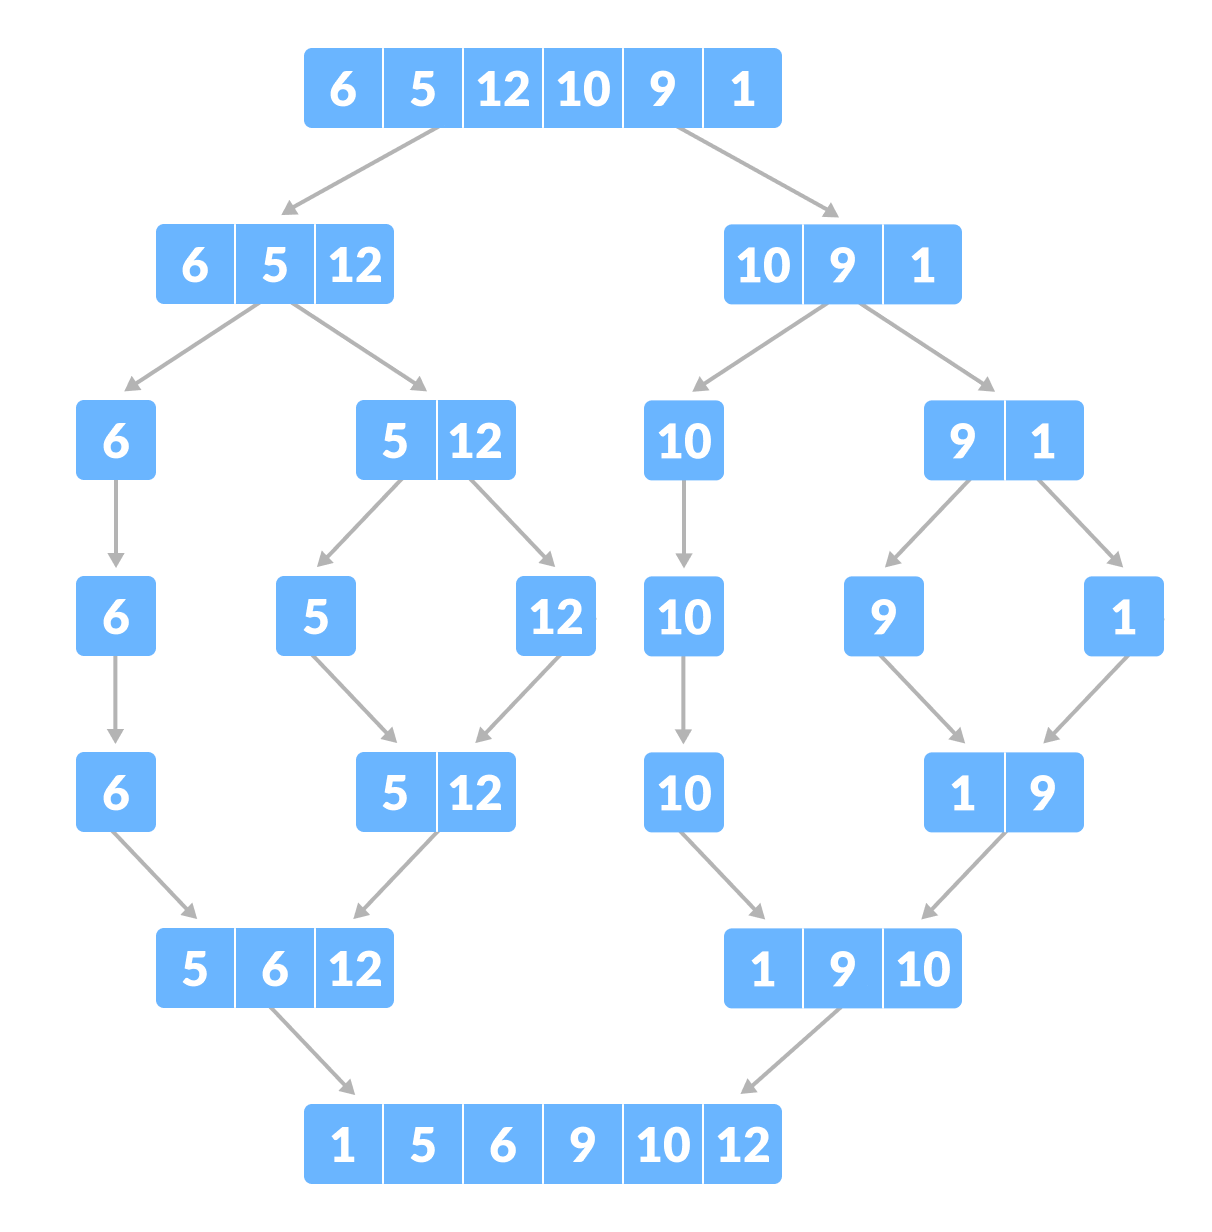
\includegraphics[scale=0.4]{figures/merge-sort-example_0.png}
	\caption{Diagrama exemplo de um Merge Sort}
	\label{fig:merge_sort_example_0}
\end{figure}

\FloatBarrier

\newpage

\subsection{Merge Sort Recursivo}

Dito isso, agora fica mais fácil estabelecer o pseudocódigo na forma recursiva. O caso base será se a lista tem no máximo um elemento, pois já está ordenada. No caso recursivo, pelo teorema da recursão temos acesso ao "caso anterior", ou seja a primeira metade e segunda metade da lista original ordenadas, portanto, podemos mesclá-las.

\begin{algorithm}
	\label{algo:merge_sort_pseudo}
	\begin{algorithmic}[1]
		\Require{$\mathbf{lista}  = x_0, x_1, \ldots, x_{N-1}$}
		\Function{MergeSort}{$\mathbf{lista}$}
		\If{tamanho da \textbf{lista} $\leq 1$} \Return
		\EndIf
		\State \Return {Merge(MergeSort($1^a$ metade da \textbf{lista}), MergeSort($2^a$ metade da \textbf{lista})}
		\EndFunction
	\end{algorithmic}
\end{algorithm}

\FloatBarrier

\subsection{Merge Sort Iterativo}

E em contraste com a abordagem anterior, a forma iterativa do Merge Sort se aproveita de estruturas de repetição aninhadas para que tenha acesso a índices específicos. E tais índices quando usados como argumento na função merge fazem com que a lista "quebrada" seja reconstruída de maneira ordenada. De forma que o loop mais externo controle a quebra da lista em sub-listas com a metade do tamanho anterior e o loop mais interno controla o índice inicial de cada sub-lista, conforme o pseudocódigo abaixo.

\begin{algorithm}
	\label{algo:merge_sort_it_pseudo}
	\begin{algorithmic}[1]
		\Require{$\mathbf{lista}  = x_0, x_1, \ldots, x_{N-1}$}
		\Function{MergeSortIt}{$\mathbf{lista}$}
		\State {tamanhoListas $\gets$ {$1$}}
		\Comment tamanho atual das sub-listas(variando de 1 até n/2)
		\State {índiceEsq $\gets$ {$1$}}
		\Comment index inicial da sub-lista à esquerda

		\For {tamanhoListas $\leq$ tamanho(\textbf{lista}) ; tamanhoListas $= 2$ $\cdot$ tamanhoListas}

		\For {índiceEsq $<$ tamanho(\textbf{lista}) $-$ $1$ ; índiceEsq $\cdot= 2$ $\cdot$ tamanhoListas}
		\State {meio $\gets$ índiceEsquerda $+$ tamanhoListas $-$ $1$}
		\State {fimDireita $\gets$ mínimo(índiceEsq $+$ $2$ $\cdot$ tamanhoListas, tamanho \textbf{lista} $-$ $1$)}
		\State {$Merge$(lista, índiceEsq, meio, fimDireita)}
		\EndFor
		\EndFor
		\EndFunction
	\end{algorithmic}
\end{algorithm}

\subsection{Função auxiliar Merge}

\noindent
Nos resta agora apenas definir a função \textbf{Merge}, que vai ser responsável por mesclar duas listas que estão ordenadas. Para tal, a função deve comparar um elemento da primeira lista com um da segunda e anexar o menor elemento entre os dois no final da lista resultado. Por exemplo:

\begin{figure}[!ht]
	\centering
	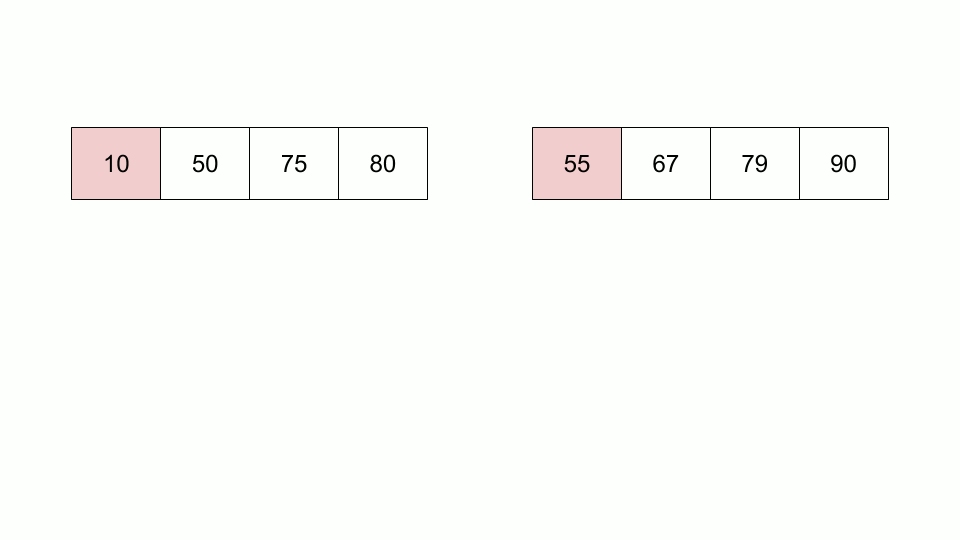
\includegraphics[scale=0.3]{figures/merge/merge-function-1.png}
	\caption{Comparando o primeiro elemento da primeira lista com o primeiro da segunda}
\end{figure}
\begin{figure}[!ht]
	\centering
	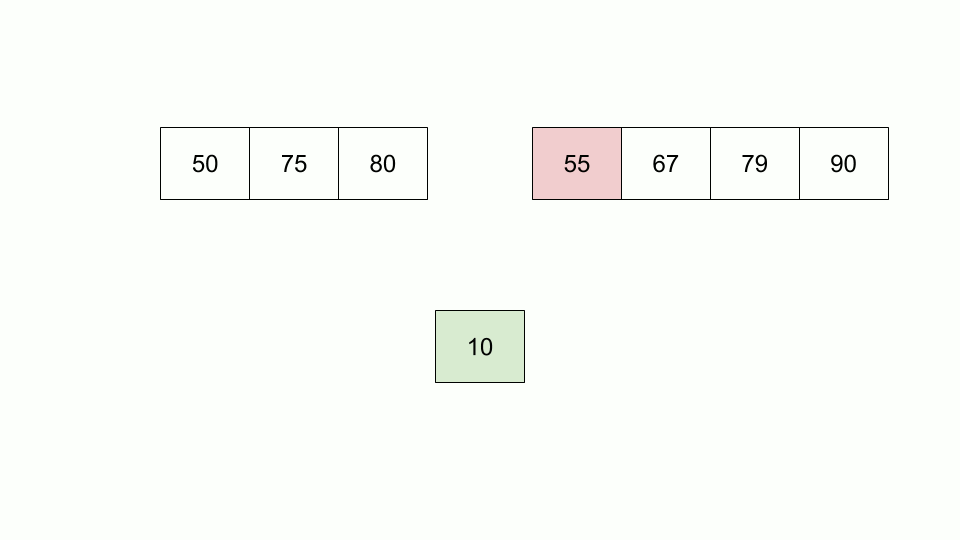
\includegraphics[scale=0.3]{figures/merge/merge-function-3.png}
	\caption{10 é menor que 55, então é anexado no final da lista resultado}
\end{figure}
\begin{figure}[!ht]
	\centering
	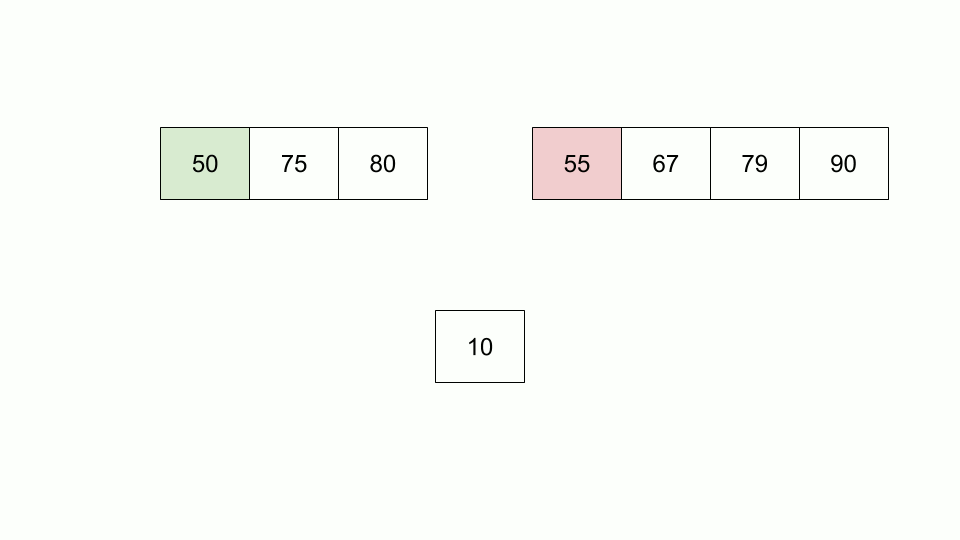
\includegraphics[scale=0.3]{figures/merge/merge-function-5.png}
	\caption{Comparando o próximo elemento da primeira lista}
\end{figure}
\begin{figure}[!ht]
	\centering
	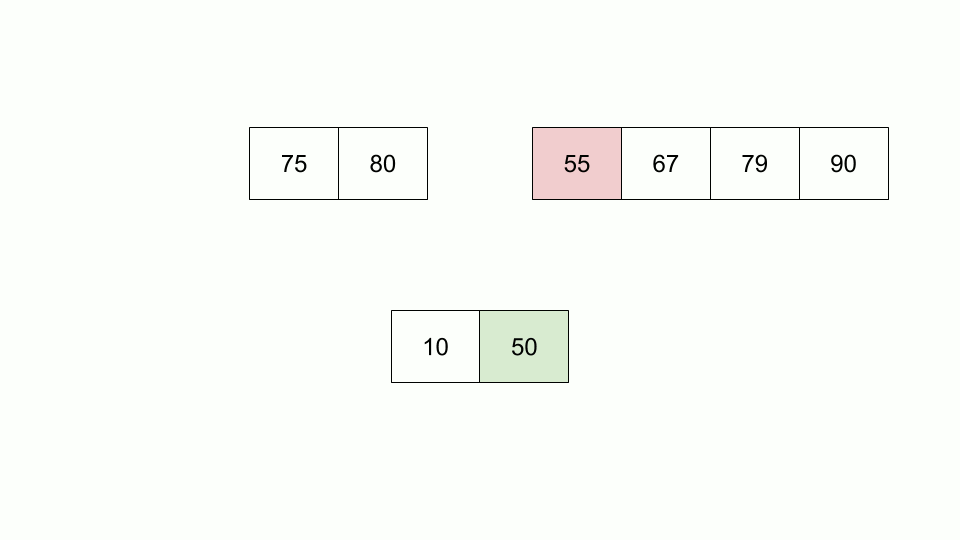
\includegraphics[scale=0.3]{figures/merge/merge-function-6.png}
	\caption{50 é menor que 55, então é anexado no final da lista resultado}
\end{figure}
\begin{figure}[!ht]
	\centering
	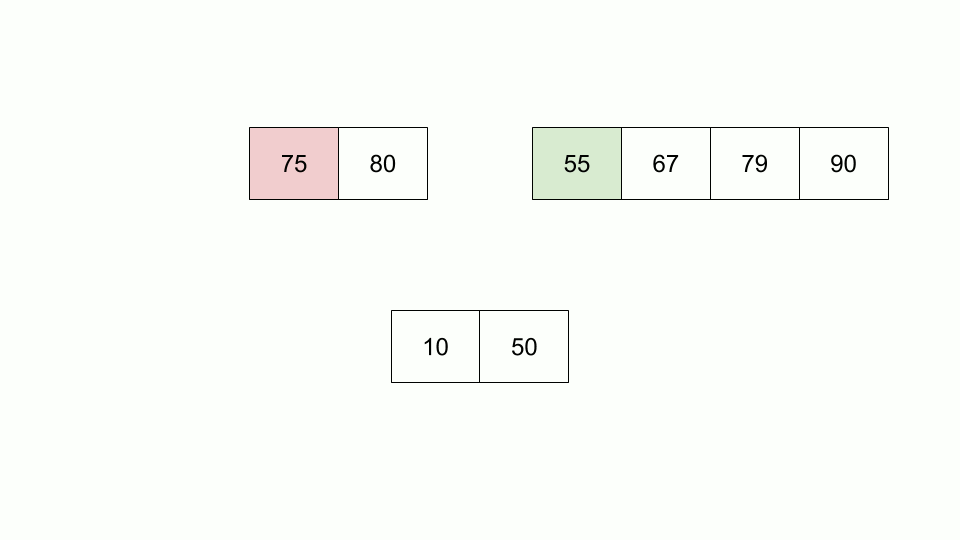
\includegraphics[scale=0.3]{figures/merge/merge-function-8.png}
	\caption{Comparando o próximo elemento da primeira lista}
\end{figure}
\begin{figure}[!ht]
	\centering
	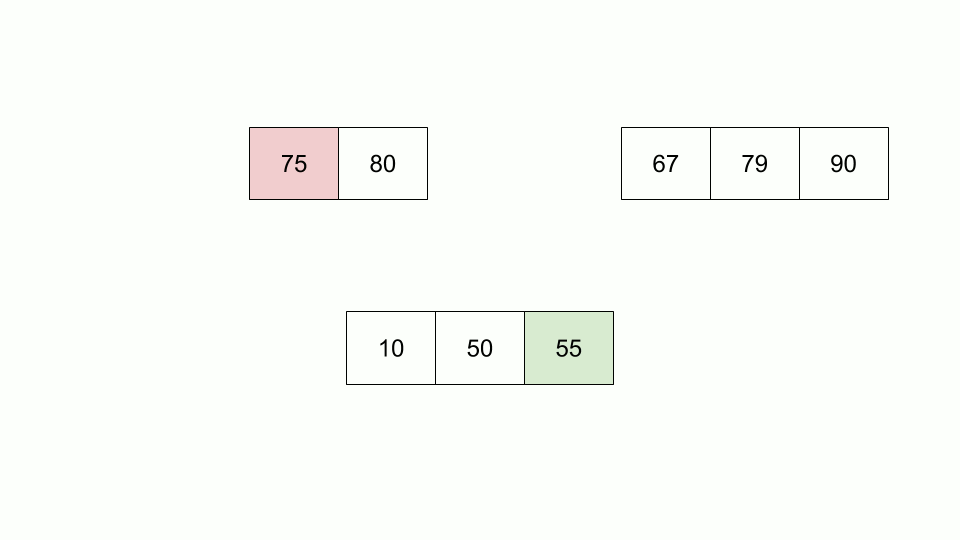
\includegraphics[scale=0.3]{figures/merge/merge-function-9.png}
	\caption{55 é menor, então é anexado no final da lista resultado}
\end{figure}
\begin{figure}[!ht]
	\centering
	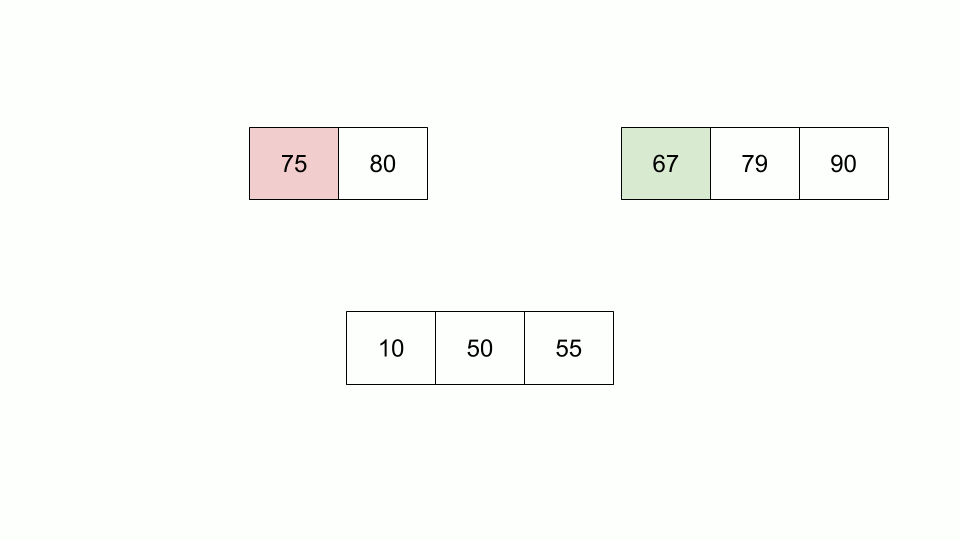
\includegraphics[scale=0.3]{figures/merge/merge-function-11.png}
	\caption{Comparando o próximo elemento da segunda lista}
\end{figure}

\FloatBarrier

E o algoritmo vai continuar até que a lista resultado esteja completa com os elementos da primeira e segunda lista.

Dito isso, construímos o pseudocódigo dessa função da seguinte forma:

\begin{algorithm}
	\label{algo:merge_aux_pseudo}
	\begin{algorithmic}[1]
		\Require{$\mathbf{listaEsquerda} = x_0, x_1, \ldots, x_{N - 1}$, $\mathbf{listaDireita} = y_0, y_1, \ldots, y_{M - 1}$}
		\Ensure{A \textbf{listaResultado} ordenada com os elementos da \textbf{listaEsquerda} e \textbf{listaDireita}}
		\Statex
		\Function{Merge}{$\mathbf{listaEsquerda}$, $\mathbf{listaDireita}$}
		\State $E, D, R \gets 0$ \Comment Esses serão os indexadores de cada lista
		\State $\mathbf{listaResultado} = 0, 0,\ldots, 0$
		\While{$E < N$ e $D < M$}
		\If{\textbf{listaEsquerda}(E) < \textbf{listaDireita}(D)}
		\State $\mathbf{listaResultado}(R).push(\mathbf{listaDireita}(D)$)
		\State $E \gets E + 1$ \Comment Partimos para o próximo elemento
		\Else
		\State $\mathbf{listaResultado}(R).push(\mathbf{listaEsquerda}(D)$)
		\State $D \gets D + 1$
		\EndIf
		\State $R \gets R + 1$
		\EndWhile
		\State $\rhd \text{ Como uma das listas vai esgotar primeiro que a outra, copiamos os elementos}$
		\State $\text{restantes para a }\mathbf{listaResultado}$
		\While {\textbf{listaEsquerda} ou \textbf{listaDireita} tiver elementos}
		\State adicione os elementos na \textbf{listaResultado}
		\EndWhile
		\State \Return \textbf{listaResultado}
		\EndFunction
	\end{algorithmic}
\end{algorithm}

\subsection{Análise de complexidade}
\label{anal:merge_sort}

Para analisar qual é a complexidade de tempo da Merge sort, nas suas duas versões, vamos estabelecer primeiro qual é a complexidade da função \textbf{Merge}. A partir do \href{algo:merge_aux_pseudo}{pseudocódigo} da função, é facil de ver que durante sua execução ela sempre vai percorrer o tamanho máximo entre a \textbf{listaEsquerda} e \textbf{listaDireita}, portanto, sua complexidade na notação de complexidade assintótica é $O(n)$, $\Theta(n)$ e $\Omega(n)$ para um tamanho de lista $n$.

\subsubsection{Análise da versão iterativa}

Observando a estrutura do \href{algo:merge_sort_it_pseudo}{pseudocódigo} dessa versão é possível perceber que ela é estritamente dependente do aninhamento de loops, e nada mais. E simplificando o algoritmo podemos observá-lo da seguinte maneira:

\begin{algorithm}
	\begin{algorithmic}[0]
		\For{$i \gets 1 ; i \leq n - 1 ; i = i \cdot 2$}
		\For{$j \gets 0 ; j < n - 1 ; j += i \cdot 2$}

		\State {$Merge()$}
		\EndFor
		\EndFor
	\end{algorithmic}
\end{algorithm}
\FloatBarrier

Além disso, a versão iterativa já começa com as sub-listas divididas em singletons a partir, restando apenas mesclar cada segmento e incrementar o seu tamanho.

\begin{algorithm}
	\begin{algorithmic}[0]
		\State $\text{tamanhoListas} \gets 1$
		\While{tamanhoListas $\leq$ tamanho(\textbf{lista}) ; tamanhoListas $= 2 \cdot$ tamanhoListas}
		\State ...
		\EndWhile
	\end{algorithmic}
\end{algorithm}

Sendo assim, apesar dos processos ocorrerem simultaneamente, podemos separar análise de complexidade da versão iterativa em duas partes: Reconstrução em sub-listas maiores e mesclagem ordenada das sub-listas.

Com a lista começando com \textbf{n} sub-listas unitárias, o primeiro passo é transformá-las em \textbf{$\frac{n}{2}$} pares, e em seguida em \textbf{$\frac{n}{4}$} quartetos, e depois em \textbf{$\frac{n}{8}$} oitavos, até obtermos uma única lista de tamanho \textbf{n}. 

Em cada iteração, o número de sublistas é dividido por 2, ou seja, o número de sublistas na iteração $i$ é dado por $\frac{n}{2^i}$. O processo continua até que haja apenas uma sublista restante, o que ocorre quando:

\begin{align*}
  \frac{n}{2^i} = 1 &\Longrightarrow n = 2^i \\
                    &\Longrightarrow \log_2 n = i
\end{align*}

Assim, o número total de iterações necessárias é $i = \log_2 n$. Como cada iteração envolve percorrer todas as sublistas para realizar as fusões, ou seja, a complexidade da função Merge, o custo de cada iteração é proporcional a \textbf{n}. Portanto, o tempo total de execução do algoritmo é:

\begin{align*}
	T(n) & = O(n) \cdot O(\log_2{n}) \\
	     & = O(n \cdot \log_2{n})
\end{align*}

Analisando da perspectiva do pior caso, perceba que mesmo se tratando de uma lista já ordenada ainda sim será necessário sub-dividí-la e reconstruí-la tal qual uma desordenada. Sendo assim, temos que a complexidade entre os cenários terá a mesma ordem independentemente do quão perto o algoritmos esteja do resultado desejado. Portanto, na notação assintótica a complexidade da Merge Sort iterativo é $O(n \cdot \log_2{n})$, $\Omega(n \cdot \log_2{n})$, $\Theta(n \cdot \log_2{n})$.

\subsubsection{Análise da versão recursiva}

Analisando o corpo da função, teremos dois casos: caso o tamanho da lista ($n$) seja menor ou igual 1 e caso contrário.

\begin{algorithm}
	\begin{algorithmic}[0]
		\If{tamanho da \textbf{lista} $\leq 1$} \Return
		\EndIf
		\State \Return {Merge(MergeSort($1^a$ metade da \textbf{lista}), MergeSort($2^a$ metade da \textbf{lista})}
	\end{algorithmic}
\end{algorithm}
\FloatBarrier

No primeiro caso, é fácil de ver que a complexidade da função para uma lista de qualquer tamanho é constante, ou seja, $O(1)$, $\Theta(1)$ e $\Omega(1)$. Caso contrário, observa-se que a função chama a si mesmo duas vezes, uma para cada metade da lista. Ademais, a função Merge, com complexidade linear para qualquer entrada, é chamada em cada etapa recursiva. Portanto, estabelecemos a relação de recorrência da Merge Sort recursiva como:


\begin{align*}
	T(n) =
	\begin{cases}
		O(1),                   & \text{se $n \leq 1$}  \\
		2T(\frac{n}{2}) + O(n), & \text{caso contrário}
	\end{cases}
\end{align*}

Uma vez estabelecida a relação de recorrência, podemos analisar a complexidade da função utilizando os quatro métodos estudados no curso. Como o Merge Sort se comporta de maneira consistente em todos os casos—melhor, pior e médio—isso simplifica nossa análise. Optaremos por começar utilizando o método da \textbf{Substituição} para determinar a complexidade.

Primeiramente, queremos demonstrar que $T(n) \geq n \cdot \log_2 n$, a fim de encontrar a complexidade na notação $\Omega$, que será equivalente às outras notações assintóticas. Por indução no $n$, teremos:

% TODO: Colocar num enumerate

\begin{itemize}
	\item Caso $n = 1$:
	      \begin{adjustwidth}{1em}{}
		      Temos que:
		      \begin{align*}
			      T(1) = 1 \text{ \& } n \cdot \log_2 1 = 0
		      \end{align*}
		      Logo $T(1) \geq n \cdot \log_2 1$.
	      \end{adjustwidth}
	\item Caso $n = k + 1$, para algum $k \in \mathbb{N}$:
	      \begin{adjustwidth}{1em}{}
		      Suponha que $T(n) \geq n \cdot \log_2 n$ (hipótese de indução). Calculemos:
		      \begin{align*}
			      T(n + 1) & = 2T\left(\frac{n + 1}{2}\right) + O(n)                                                                                            \\
			               & \geq 2 \cdot \frac{n + 1}{2} \cdot \log_2 \left(\frac{n + 1}{2}\right) + O(n) &  & \text{(hipótese de indução e função crescente)} \\
			               & = (n + 1)(\log_2 (n + 1) - 1) + O(n)                                                                                               \\
			               & = (n + 1)\log_2 (n + 1)) - n + 1 + O(n)                                                                                            \\
			               & \geq (n + 1)\log_2 (n + 1)
		      \end{align*}
		      Dessa forma $T(n + 1) \geq (n + 1)\log_2 (n + 1)$.
	      \end{adjustwidth}
\end{itemize}

Como também sabemos que o Merge Sort não excede $O(n \cdot \log_2 n)$ em termos de complexidade, podemos concluir que:

\begin{align*}
  T(n) = \Theta(n \cdot \log_2 n)
\end{align*}

Após analisar o Merge Sort pelo método da substituição, vamos dar continuidade ao nosso exercício ao analisá-lo pelo método da \textbf{Iteração}. Para tal, começaremos expandimos a recorrência até um padrão ser identificado:

\begin{align*}
	T(n) & =  2T\left(\frac{n}{2}\right) + n     \\
	     & = 4T\left(\frac{n}{2}\right) + 2n     \\
	     & = 8T\left(\frac{n}{2}\right) + 4n     \\
	     & \vdots                                \\
	     & = 2^iT\left(\frac{n}{2^i}\right) + in \\
\end{align*}

Dessa forma, é identificado o caso base da relação a partir de:

\begin{align*}
	\frac{n}{2^i} = 1 & \Longrightarrow n = 2^i      \\
	                  & \Longrightarrow \log_2 n = i
\end{align*}

Substituindo, temos que:

\begin{align*}
	 & = n \cdot T(1) + n \cdot \log_2 n \\
	 & = n + n \cdot \log_2 n
\end{align*}

Portanto, a complexidade do Merge Sort se mantém consistente com o método da substituição e tem complexidade $n \cdot \log_2 n$ nas notações assintóticas.

Agora, vamos usar o método da \textbf{Árvore de recorrência} para verificar o mesmo resultado. Comecemos estabelecendo a árvore de recursão:


\[\begin{tikzcd}[sep=small]
		&&&& {T(n)} \\
		\\
		&& {T(\frac{n}{2})} &&&& {T(\frac{n}{2})} \\
		& {T(\frac{n}{4})} & {T(\frac{n}{4})} &&&& {T(\frac{n}{4})} & {T(\frac{n}{4})} \\
		{T(\frac{n}{8})} & {T(\frac{n}{8})} & {T(\frac{n}{8})} & {T(\frac{n}{8})} && {T(\frac{n}{8})} & {T(\frac{n}{8})} & {T(\frac{n}{8})} & {T(\frac{n}{8})} \\
		\vdots & \vdots & \vdots & \vdots & \vdots & \vdots & \vdots & \vdots & \vdots
		\arrow[from=1-5, to=3-3]
		\arrow[from=1-5, to=3-7]
		\arrow[from=3-3, to=4-2]
		\arrow[from=3-3, to=4-3]
		\arrow[from=3-7, to=4-7]
		\arrow[from=3-7, to=4-8]
		\arrow[from=4-2, to=5-1]
		\arrow[from=4-2, to=5-2]
		\arrow[from=4-3, to=5-3]
		\arrow[from=4-3, to=5-4]
		\arrow[from=4-7, to=5-6]
		\arrow[from=4-7, to=5-7]
		\arrow[from=4-8, to=5-8]
		\arrow[from=4-8, to=5-9]
	\end{tikzcd}\]
\FloatBarrier

Uma vez estabelecida a árvore de recorrência, podemos tabular o tamanho da entrada, seu custo por nó e quantidade de nós para cada nível da árvore:


\begin{table}[h!]
	\centering
	\begin{tabular}{lrrr}
		\toprule
		Nível da árvore & Tamanho da entrada & Custo por nó    & Quantidade de nós \\
		\midrule
		0               & $n$                & n               & $1 = 2^0$         \\
		1               & $\frac{n}{2^1}$    & $\frac{n}{2^1}$ & $2 = 2^1$         \\
		2               & $\frac{n}{2^2}$    & $\frac{n}{2^2}$ & $4 = 2^2$         \\
		3               & $\frac{n}{2^3}$    & $\frac{n}{2^3}$ & $8 = 2^3$         \\
		$\vdots$        & $\vdots$           & \vdots          & \vdots            \\
		i               & $\frac{n}{2^i}$    & $\frac{n}{2^i}$ & $2^i$             \\
		\bottomrule
	\end{tabular}
\end{table}
\FloatBarrier

Em seguida, para estabelecer o somatório que calcula a complexidade da função, precisamos identificar o valor de $i$ para quando $T(\frac{n}{2^i}) = T(1)$, assim, teremos:

\begin{align*}
	\frac{n}{2^i} = 1 & \Longrightarrow n = 2^i      \\
	                  & \Longrightarrow \log_2 n = i
\end{align*}

Dessa forma, a complexidade da função para $\Omega$, $\Theta$ e $O$ será dada pelo resultado do somatório:

\begin{align*}
	\sum_{i = 0}^{\log_2 n} \frac{n}{2^i} \cdot 2^i & = \sum_{i = 0}^{\log_2 n}n  \\
	                                                & = n\sum_{i = 0}^{\log_2 n}1 \\
	                                                & = n \cdot \log_2 n
\end{align*}


Pelo método do \textbf{Teorema mestre}, o mesmo resultado ocorre em ainda menos etapas. Pelo teorema, temos que estabelecendo a relação de recorrência nessa forma:

$$
	T(n) = aT\left(\frac{n}{b}\right) + \Theta\left(n^{k}\right)
$$

Para algum $a \geq 1$, $b \geq 1$, e $k \geq 0$. Vale que:

\begin{enumerate}
	\item Se $a \geq b^k$, então $T(n)$ é $\Theta(n^{\log_b a})$.
	\item Se $a = b^k$, então $T(n)$ é $\Theta(n^k \cdot \log_b a)$.
	\item Se $a < b^k$, então $T(n)$ é $\Theta(n^k)$.
\end{enumerate}

A partir da \href{recc:rec_merge_sort}{relação de recorrência estabelecida}, tome $a = 2$, $b = 2$ e $k = 1$. Como $b^k = 2 = a$, logo, $T(n) = \Theta(n \cdot \log_2 n)$. Como foi estabelecido que o pior caso, o melhor e caso médio iam ter a mesma complexidade, logo, a \textit{Merge sort} também tem as complexidades $O(n \cdot \log_2 n)$ e $\Omega(n \cdot \log_2 n)$. E aqui terminamos essa análise.


\newpage

\section{Quick Sort}
\label{sec:quick-sort-teo}

Assim como o Merge Sort, o Quick Sort é um algoritmo baseado na técnica de divisão e conquista. A operação ocorre da seguinte forma:

\begin{enumerate}
	\item \textbf{Dividir}: O vetor \( A[p..r] \) é dividido em dois subvetores não vazios \( A[p..q] \) e \( A[q+1..r] \). O índice \( q \) é escolhido a partir do elemento localizado na metade do vetor original, denominado pivô. Os elementos do vetor são rearranjados de modo que os elementos à esquerda de \( q \) sejam menores ou iguais ao pivô, e os elementos à direita sejam maiores ou iguais ao pivô.

	\item \textbf{Conquistar}: Os dois subvetores \( A[p..q] \) e \( A[q+1..r] \) são ordenados através de chamadas recursivas ao Quick Sort.

	\item \textbf{Combinar}: Esta etapa não exige nenhum processamento adicional, pois, ao longo do processo recursivo, os elementos vão sendo ordenados no próprio vetor.
\end{enumerate}

Para um melhor entendimento, segue uma esquema do primeiro laço de repetição realizado por este algoritmo:

\begin{figure}[!ht]
	\centering
	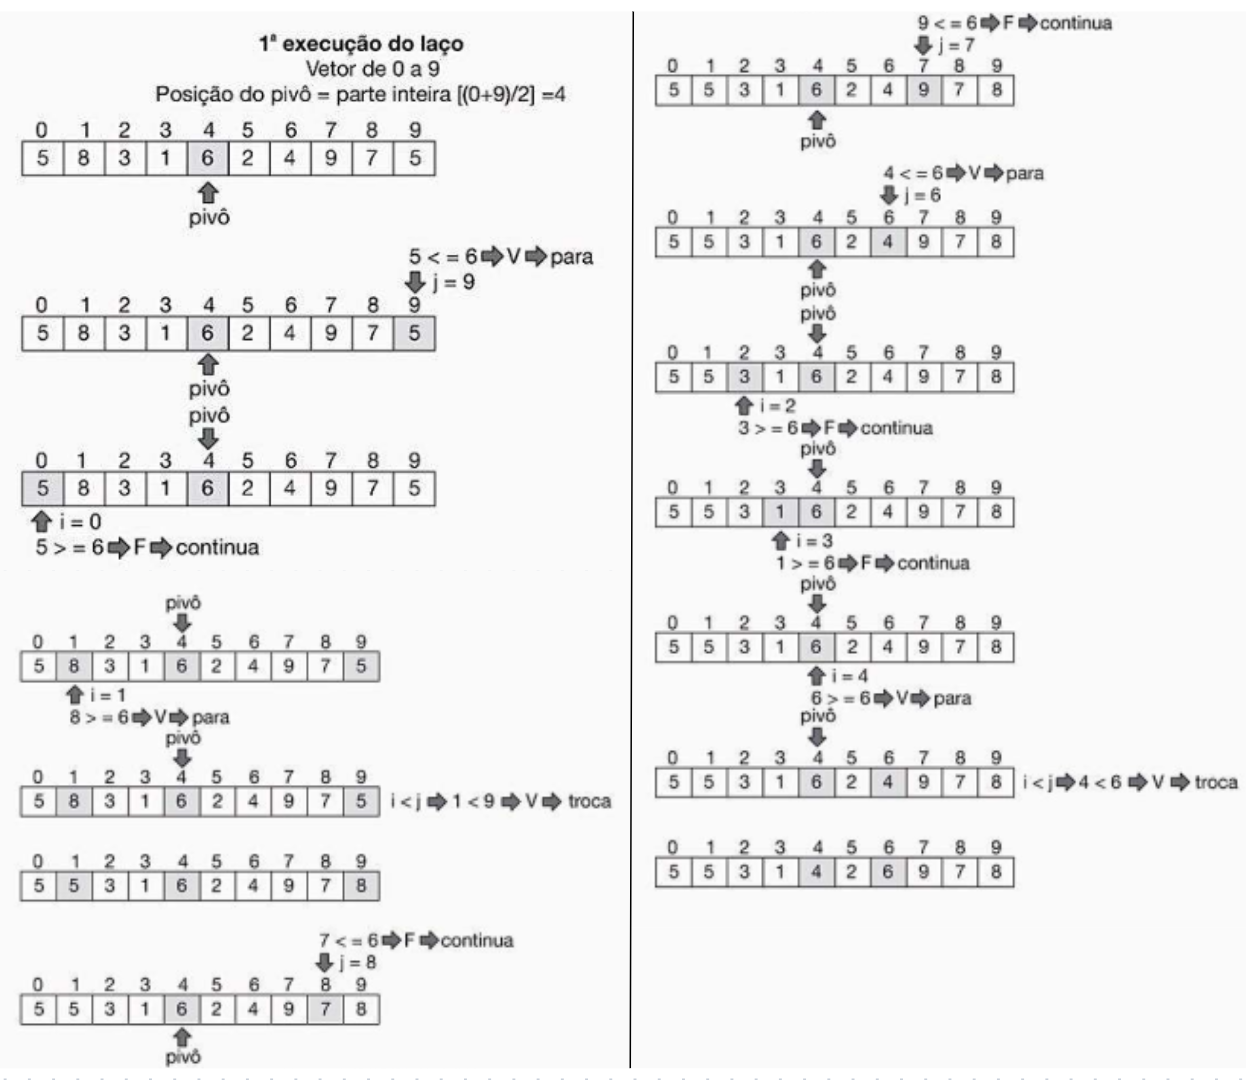
\includegraphics[scale=0.34]{figures/quick/q1.png}
	\caption{Disponível em: ASCÊNCIO, Ana Fernanda Gomes; ARAÚJO, Graziela Santos. Estruturas de Dados: Algoritmos, Análise da Complexidade e Implementações em Java e C/C++.  Pearson; 1ª edição (30 setembro 2015)}
	\label{fig:quick_sort_example}
\end{figure}
\FloatBarrier

\subsection{Quick Sort Recursivo}

Portanto, o caso base da Quick sort recursiva será o intervalo a ser ordenado for tiver 1 elemento ou for vazio. E a etapa recursiva será a chamada da função para a primeira metade até o pivô e segunda metade até o fim da lista.

\begin{algorithm}
	\caption{Quick Sort Recursivo}
	\label{algo:rec_quick_sort}
	\begin{algorithmic}[1]
		\Function{QuickSortRecursivo}{A, limiteEsquerdo, limiteDireito}
		\If{$\text{limiteEsquerdo} \geq \text{limiteDireito}$}
		\Return
		\EndIf
		\State $\text{indicePivot} \gets$ \Call{particao}{$A, \text{limiteEsquerdo}, \text{limiteDireito}$}
		\State \Call{quickSort}{$A, \text{limiteEsquerdo}, \text{indicePivot}$}
		\State \Call{quickSort}{$A, q+1, r$}
		\EndFunction
	\end{algorithmic}
\end{algorithm}
\FloatBarrier

\subsection{Quick Sort Iterativo}

Dado que o Quick Sort é um algoritmo naturalmente recursivo, vamos emular a pilha de execução do computador usando a estrutura de dados pilha, cada chamada recursiva vai ser uma inserção na pilha, e cada etapa de execução será uma remoção na pilha. Com essas considerações, podemos copiar e colar o resto da implementação recursiva.

\begin{algorithm}
	\caption{Iterative Quick Sort}
	\label{algo:iterative_quick_sort}
	\begin{algorithmic}[1]
		\Require{Lista $A$}
		\Ensure{Lista $A$ ordenada}
		\Statex

		\Function{IterativeQuickSort}{$A$}
		\If{$A$ estiver vazio}
		\State \Return
		\EndIf
		\State Crie uma pilha com o par $(0, \text{tamanho de } A - 1)$

		\While{a pilha não estiver vazia}
		\State Remova $(\text{limiteEsquerdo}, \text{limiteDireito})$ do topo da pilha

		\If{$\text{limiteEsquerdo} \geq \text{limiteDireito}$}
		\State \textbf{continue}
		\EndIf
		\State Adicione $(\text{limiteEsquerdo}, \text{indicePivot} - 1)$ na pilha \Comment{Lado esquerdo}
		\State Adicione $(\text{indicePivot} + 1, \text{limiteDireito})$ na pilha \Comment{Lado direito}
		\EndWhile
		\EndFunction
	\end{algorithmic}
\end{algorithm}
\FloatBarrier
\newpage

\subsection{Função auxiliar Partição}

A função partição é responsável pela maior parte do trabalho braçal do Quick Sort, ela é quem organiza uma lista em relação a dterminado pivô

\begin{algorithm}
	\caption{Partição}
	\label{algo:particao}
	\begin{algorithmic}[1]
		\Require{A = $a_1, a_2, a_3, \ldots, a_n$, limiteEsquerdo, limiteDireito}
		\Ensure{O índice do pivô}
		\Function{particao}{$A, \text{limiteEsquerdo}, \text{limiteDireito}$}
		\State pivô $\gets A[\text{limiteDireito}]$
		\State itemEsquerdo $\gets \text{limiteEsquerdo}$
		\For{itemDireito $\gets$ limiteEsquerdo to limiteDireito}
		\If{$A[\text{itemDireito}] <$ pivô}
		\State \textbf{troque} itemDireito por itemDireito em $A$
		\State itemEsquerdo $\gets$ itemEsquerdo $+ 1$
		\EndIf
		\EndFor
		\State \textbf{troque} itemEsquerdo por limiteDireito em A \Comment O pivô é colocado no meio
		\State \Return itemEsquerdo
		\EndFunction
	\end{algorithmic}
\end{algorithm}
\FloatBarrier

\subsection{Análise de Complexidade}

\subsubsection{Análise da versão recursiva}

Primeiro, devemos definir a relação de recorrência do algoritmo.

No procedimento de partição, o tempo de execução é limitado pelo tamanho \( n \) do vetor. Isso ocorre porque ele compara todos os elementos do vetor com o pivô enquanto os índices atenderem a condição \( i < j \). Logo, o procedimento de partição realizará \( O(n) \) comparações.

Os dois vetores gerados pelo procedimento de partição são resolvidos recursivamente. O tamanho desses vetores depende do valor do pivô escolhido na função de partição. Suponha que \( k \) elementos estejam ao lado esquerdo do pivô e \( (n - k - 1) \) elementos estejam à direita do pivô após a partição.

Logo, a complexidade do passo recursivo será a soma das recorrências da ordenação dos dois vetores: \( T(k) + T(n - k - 1) \).

Somando a parte recursiva do algoritmo com o procedimento de partição, teremos:
\[
	T(n) = O(n) + T(k) + T(n - k - 1)
\]

O tempo de execução do Quick Sort depende se o particionamento é ou não balanceado. Se for balanceado, o algoritmo executa tão rapidamente quanto o Merge Sort; caso contrário, ele executará tão lentamente quanto o Insertion Sort. Assim, temos dois casos:

\begin{itemize}
	\item \textbf{Pior caso:} Ocorre quando o pivô é o maior ou o menor elemento do vetor. Aqui, um vetor terá \( n-1 \) elementos e o outro vetor será vazio (não se esqueça do pivô).

	      Para calcular a complexidade do Quick Sort no pior caso, substituímos \( k = n - 1 \) na recorrência encontrada:
	      \[
		      T(n) = O(n) + T(n-1) + T(n - n + 1 - 1)
	      \]
	      \[
		      = cn + T(n-1) \quad \text{(considere \( c \) uma constante)}
	      \]

	      Observe que, neste caso, o algoritmo se comportará da mesma forma que o BubbleSort, que já foi analisado neste trabalho.

	\item \textbf{Melhor caso:} Ocorre quando o pivô é o elemento médio do vetor a ser ordenado em cada chamada do algoritmo de partição. Nessa situação, o processo de partição será balanceado e o tamanho de cada vetor gerado pela partição será, aproximadamente, \( n/2 \).

	      Para calcular a complexidade do Quick Sort nesse caso, substituímos \( k = n/2 \) na recorrência encontrada:
	      \[
		      T(n) = O(n) + T(n/2) + T(n - n/2 - 1)
	      \]
	      \[
		      \approx cn + 2T(n/2)
	      \]

	      Agora, note que o Quick Sort, em seu melhor caso, se comporta da mesma forma do Merge Sort (\ref{sec:merge-sort-teo}), dessa forma sua complexidade no melhor caso é $\Omega(n \cdot \log_2 n)$.

\end{itemize}

\subsubsection{Análise da versão iterativa}

Para determinar a complexidade da versão iterativa, precisamos estimar o tamanho da estrutura de dados "pilha" que simula as chamadas recursivas da outra versão. De forma que seja compreendido quando a estrutura de repetição "while" vai parar. Para tal, teremos dois casos:

\begin{itemize}
	\item \textbf{Melhor caso}: Vamos supor que a função "partição"  sempre particione a lista em duas sublistas iguais, ou seja, o pivô escolhido é sempre a mediana da lista maior, de forma que:
	      \begin{adjustwidth}{-1.8em}{}
		      \begin{tikzcd}[sep=small]
			      &&&& n &&&&& cn \\
			      \\
			      &&& {n/2} && {n/2} &&&& {2 \cdot cn/2 =cn} \\
			      \\
			      & {n/4} && {n/4} && {n/4} && {n/4} && {4 \cdot cn/4 = cn} \\
			      \\
			      {n/8} & {n/8} & {n/8} & {n/8} && {n/8} & {n/8} & {n/8} & {n/8} & {8 \cdot cn/8 = cn} \\
			      \vdots & \vdots & \vdots & \vdots && \vdots & \vdots & \vdots & \vdots \\
			      1 & 1 & 1 & 1 && 1 & 1 & 1 & 1 & {n \cdot c = cn}
			      \arrow[from=1-5, to=3-4]
			      \arrow[from=1-5, to=3-6]
			      \arrow[from=3-4, to=5-2]
			      \arrow[from=3-4, to=5-4]
			      \arrow[from=3-6, to=5-6]
			      \arrow[from=3-6, to=5-8]
			      \arrow[from=5-2, to=7-1]
			      \arrow[from=5-2, to=7-2]
			      \arrow[from=5-4, to=7-3]
			      \arrow[from=5-4, to=7-4]
			      \arrow[from=5-6, to=7-6]
			      \arrow[from=5-6, to=7-7]
			      \arrow[from=5-8, to=7-8]
			      \arrow[from=5-8, to=7-9]
		      \end{tikzcd}
	      \end{adjustwidth}

	      Assim, a recorrência continuará até que \( \frac{n}{2^i} = 1 \), com \( i \) representando o nível da árvore representada acima. Com isso, teremos:

	      \[
		      n = 2^i \implies i = \log_2 n
	      \]

	      Ou seja, a árvore terá \( \log_2 n \) níveis, e cada nível da árvore de recursão realiza um trabalho proporcional a \( n \), devido ao processo de particionamento. Portanto, a complexidade nesse caso será dada por \( T(n) = n \log_2 n \).

	      Assim, podemos dizer que o tempo de execução do algoritmo Quick Sort, em sua forma iterativa no melhor caso, será \( O(n \log n) \), pois:

	      \[
		      \lim_{n \rightarrow \infty} \frac{n \cdot \log_2 n}{n \cdot \log_2 n} =
		      \lim_{n \rightarrow \infty} 1 =
		      1 \in \mathbb{R}^*_+.
	      \]

	      De forma análoga, podemos dizer que este algoritmo será \( \Omega(n \cdot \log_2 n) \) e \( \Theta(n \cdot \log_2 n) \).


	\item \textbf{Pior caso}: Como dito anteiormente, nesse caso, a função partição sempre divide a lista de forma desequilibrada, com o pivô sendo o maior ou o menor elemento do vetor. Nesse cenário, uma das sublistas contém apenas um elemento enquanto a outra contém quase todos os demais. Dessa forma, o particionamento acontece com divisões cada vez menores, resultando em uma árvore de recursão linear, como segue:

	      \[
		      \begin{tikzcd}[sep=small]
			      &&&& n &&&& cn \\
			      &&&& {n - 1} &&&& {c(n - 1)} \\
			      &&&& {n - 2} &&&& {c(n - 2)} \\
			      &&&& \vdots \\
			      &&&& 1 &&&& c
		      \end{tikzcd}
	      \]

	      Neste caso, a altura da árvore de recursão é \( n \), já que em cada nível apenas um elemento é fixado na posição correta, e as sublistas vão sendo reduzidas em apenas um elemento a cada iteração.

	      Assim, o trabalho total realizado por nível é proporcional ao tamanho da lista em cada iteração, somando-se ao longo da altura da árvore. Portanto, a complexidade total é a soma dos primeiros \( n \) números, ou seja:

	      \[
		      T(n) = n + (n - 1) + (n - 2) + \dots + 1 = \frac{n(n + 1)}{2} = \frac{n^2 + n}{2} \approx \frac{n^2}{2}
	      \]

	      Agora, observe que:
	      \[
		      \lim_{n \rightarrow \infty} \frac{\frac{n^2}{2}}{n^2} =
		      \lim_{n \rightarrow \infty} \frac{1}{2} =
		      \frac{1}{2} \in \mathbb{R}^*_+.
	      \]

	      Assim, podemos afirmar que o tempo de execução do Quick Sort, em sua forma iterativa no pior caso, é \( O(n^2) \), \( \Omega(n^2) \) e \( \Theta(n^2) \)


\end{itemize}

\newpage
